%!TEX root = main.tex
\newpage
\section{System}
\subsection{System Architecture}
\agp{stay consistent with terminology: lattice, hierarchy, graph?}
We have implemented \system\ as a web-based tool on top of a PostgreSQL database. In Figure \label{system_architecture}, we present the system architecture of \system, which consists of three core modules: the traversal module, the query module, and the statistics module. The traversal module contains several alternative algorithms for traversing the visualization hierarchy. These algorithms are responsible for both generating the visualization hierarchy and picking visualizations for the dashboard from the hierarchy. For generating the visualization hierarchy, the traversal module passes a list of data subsets corresponding to visualizations to be generated to the query module. The query module translates these visualizations into queries, and then optimizes (by grouping) and executes the queries. The statistics module is an optional module that allows the traversal module to prune low-utility visualizations without actually generating them. Specifically, it generates coarse statistics for the unexplored visualizations based on the current list of explored visualizations. 
\agp{Give forward pointers to sections that describe this.}
\begin{center}
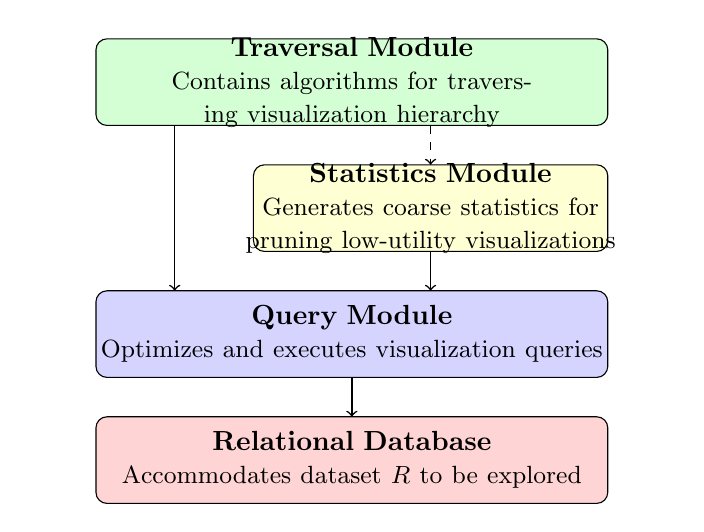
\begin{tikzpicture}
    \filldraw [fill={rgb:red,1;white,5}, rounded corners=4pt] (0, 0) rectangle (6.5, 1.1) node[pos=.5, align=center, text width=8cm] {\textbf{Relational Database}\\ {\small Accommodates dataset $R$ to be explored}};
    \filldraw [fill={rgb:blue,1;white,5}, rounded corners=4pt] (0, 1.6) rectangle (6.5, 2.7) node[pos=.5, align=center, text width=8cm] {\textbf{Query Module}\\ {\small Optimizes and executes visualization queries}};
    \filldraw [fill={rgb:yellow,1;white,5}, rounded corners=4pt] (2, 3.2) rectangle (6.5, 4.3) node[pos=.5, align=center, text width=5cm] {\textbf{Statistics Module}\\ {\small Generates coarse statistics for pruning low-utility visualizations}};
    \filldraw [fill={rgb:green,1;white,5}, rounded corners=4pt] (0, 4.8) rectangle (6.5, 5.9) node[pos=.5, align=center, text width=8cm] {\textbf{Traversal Module}\\ {\small Contains algorithms for traversing visualization hierarchy}};
    \draw [->, line width=0.2mm] (1, 4.8) -- (1, 2.7);
    \draw [->, dashed, line width=0.2mm] (4.25, 4.8) -- (4.25, 4.3);
    \draw [->, line width=0.2mm] (4.25, 3.2) -- (4.25, 2.7);
    \draw [->, line width=0.2mm] (3.25, 1.6) -- (3.25, 1.1);
\end{tikzpicture}
\label{system_architecture}
\end{center}

\subsection{Algorithms\label{algorithms}}
We give an overview of our algorithms by first discussing the approaches to generate the visualization hierarchy, and then presenting a high-level overview of our traversal algorithms.

\textbf{Lattice Generation.} Our system supports two variants of traversal algorithms based on the hierarchy generation procedure---offline variants that first generate the complete hierarchy and then work towards identifying the maximum utility solution, and online variants that incrementally generate the hierarchy and simultaneously identify the solution. The offline variants are appropriate for datasets with a small number of low-cardinality attributes, where we can generate the entire hierarchy in a reasonable time; whereas the online variants are appropriate for datasets with large number of high-cardinality attributes, where we incrementally generate a partial hierarchy. 

%In most cases, the hierarchy contains a large number of visualizations due to the presence of many attributes or high-cardinality attributes in the dataset. In such cases finding an optimal solution is computationally challenging.

\textbf{Lattice Traversal.} Given the materialized lattice, the objective of the traversal algorithm is to find the connected subgraph in the lattice that has the maximum combined edge utility. This problem known as the maximum-weight connected subgraph problem\cite{ErnstAlthaus2009} and is known to be NP-Complete, via a reduction from the \textsc{Clique Problem}\dor{cite or refer to proof in tech report}. Therefore, we focus on devising heuristic algorithms to acquire a locally optimal solution. In the following section, we will discuss the \textit{frontier greedy} algorithm which is used for generating the dashboards for our user study and defer our discussion on the details of other algorithms that we have developed to the technical report.%We devised two classes of heuristics algorithms, namely, frontier-based algorithms, and path-merging algorithms. These algorithms are guaranteed to find a solution that satisfies the constraints of our problem, except for the optimality. 
\techreport{The frontier-based algorithms traverse the hierarchy from root to downwards, incrementally adding new nodes (visualizations) to the current solution (dashboard) till it reaches the maximum capacity $k$. To achieve this, the algorithms maintain a list of candidate nodes---called \textit{frontier} nodes---any of which can be added to the current solution since their informative parent is already present in the solution. At each step, the algorithms add a node from frontier to the current solution, and update the frontier accordingly.  The frontier based algorithms can be further categorized into three types based on their node selection strategy (from frontier), namely greedy algorithm, random walk algorithm, and probabilistic algorithm. The greedy algorithm picks the current best node from frontier (thus concentrates on exploitation), random walk algorithm picks a random node (thus concentrates on exploration), and probabilistic algorithm picks a random high-utility node (thus trades off between exploration and exploitation).}
\par Our algorithm maintain a list of candidate nodes known as the \textit{frontier} nodes, which encompasses all neighbors of nodes in the existing subgraph solution. Any of the nodes in the frontier can be added to the current solution since their informative parent is guaranteed to be present in the solution. At each step, our algorithm greedily picks the node with the maximum utility from the frontier to the current solution, and updates the frontier accordingly. 
\dor{cut down on details according to aditya's comments. Need to possibly add a figure illustrating idea of "frontier". Himel needs to add pseudocode here.}
\techreport{The path merging algorithm first generate the informative paths from root to every candidate node. Then, it greedily merges the paths with high-utility to create a subgraph whose size is less than or equal to maximum capacity $k$.}
\iffalse
\begin{algorithm}
    \SetKwInOut{Input}{Input}
    \SetKwInOut{Output}{Output}
    \Input{}
    \Output{}
    \eIf{$b=0$}
      {
        return $a$\;
      }
      {
        return Euclid$(b,a\mod b)$\;
      }
    \caption{Frontier Based Algorithm}
\end{algorithm}
\fi

%\textbf{Greedy Algorithms:} Greedy algorithms select the locally optimal node to be added to the frontier. 

%A specific implementation would need to specify a scoring function to nodes in frontier that is used to pop out the next node in each iteration. One can design a scoring function based on the trade-off between performance and complexity. In the most simple case, we can use the edge weights to score nodes in the frontier. That is, at each point we add a node with the highest interestingness value. We note that this is quite a greedy approach. Specifically, we might miss visualizations with high utility that are in deeper levels of the graph. Thus, another approach would be to extent the horizon for which we calculate a nodes utility. We denote such approach as a look-ahead approach. With a free parameter $n$, we would like to assign a score to each frontier node the corresponds to the expected utility of adding this node and $n-1$ more nodes who are its descendants. For example, we can run BFP for each node in frontier treating it as a root. 


\subsection{User Interaction}
\begin{figure}[ht!]
\centering
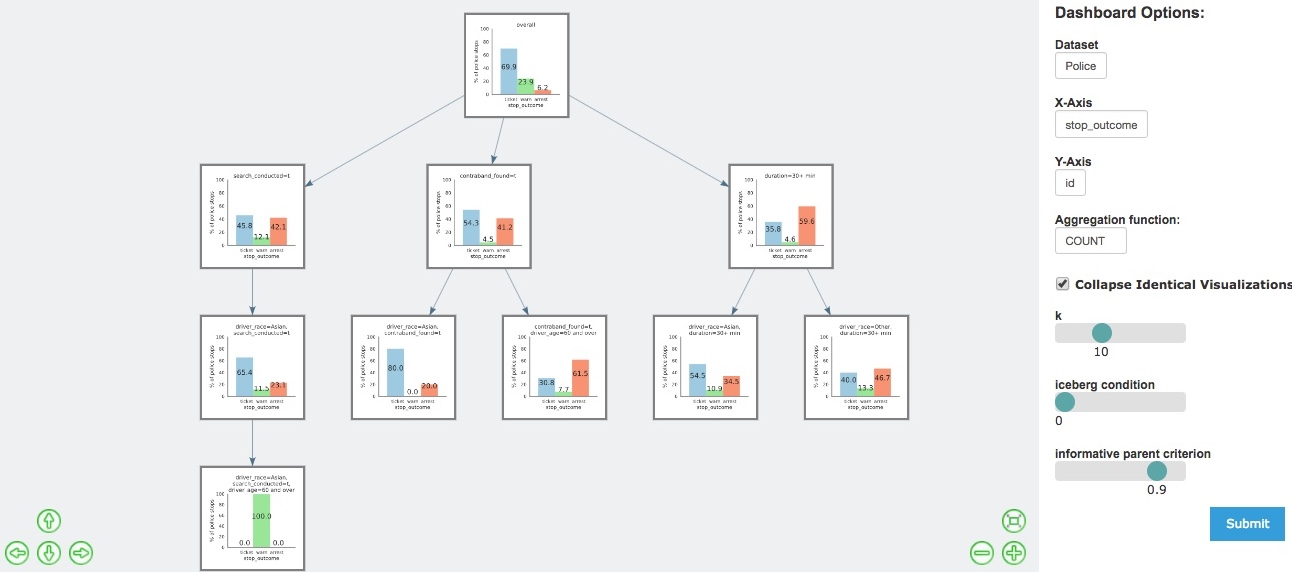
\includegraphics[width=\linewidth]{figures/overview.jpeg}
\caption{Overview of the \system interface for the Police Dataset. Users can select x and y axes of interest, as well as a choice of an aggregation function (COUNT,SUM,AVRG). Default values are set for system related parameters such as the number of visualizations to show in the dashboard (k), iceberg criterion for pruning, and informative parent criterion, which can be adjusted by the users via the sliders if needed.}
\label{fig:overview}
\end{figure}
\par Figure \ref{fig:overview} shows an overview of the \system interface. After the user selects the x and y axes of interest, aggregation function, and optional system parameter settings, an initial dashboard of $k$ visualizations is displayed on the canvas, such as the one seen in main canvas of Figure \ref{fig:overview}. The system provides toolbar buttons with keyboard binding for zooming in, out, and extent, as well as moving around the canvas. Alternatively, participants can also zoom and pan with mouse click and scroll.
\par After browsing through the visualizations the dashboard, users may be interested in getting more information about a particular node. \system supports a mechanism for users to request additional summarizations based on a chosen node of interest. As shown in Figure \ref{fig:altroot_expansion}, the analyst starts with k=5 visualizations. He learns that for the drivers who had contraband found in the vehicle, the arrest rate for drivers who are 60 and over is surprisingly higher than usual, whereas for Asian drivers the arrest rate is lower. Apart from the contraband found stories, he is also interested in learning more about the other factor that contribute to high arrest rate: duration=30+min. He clicks on the corresponding visualization and requests for 2 additional visualizations. Upon seeing the updated dashboard, he learns that unlike the contraband found story, the child distributions of the duration=30+min distribution largely follows its parent distribution, which implies that if a police stop last more than 30 minutes, the outcome would more or less be the same, independent of other factors, such as driver's race or age. The system uses the same models and algorithms as discussed earlier to generate the expansion dashboard, with the only difference that the starting node is now the selected visualization, rather than the overall visualization. This node expansion capability is similarly motivated by the idea of \textit{iterative view refinement} in other visual analytics system\cite{Wongsuphasawat2016,Hoque2017}, which is essential for the users to iterate on and explore different hypotheses. 
\begin{figure}[ht!]
\centering
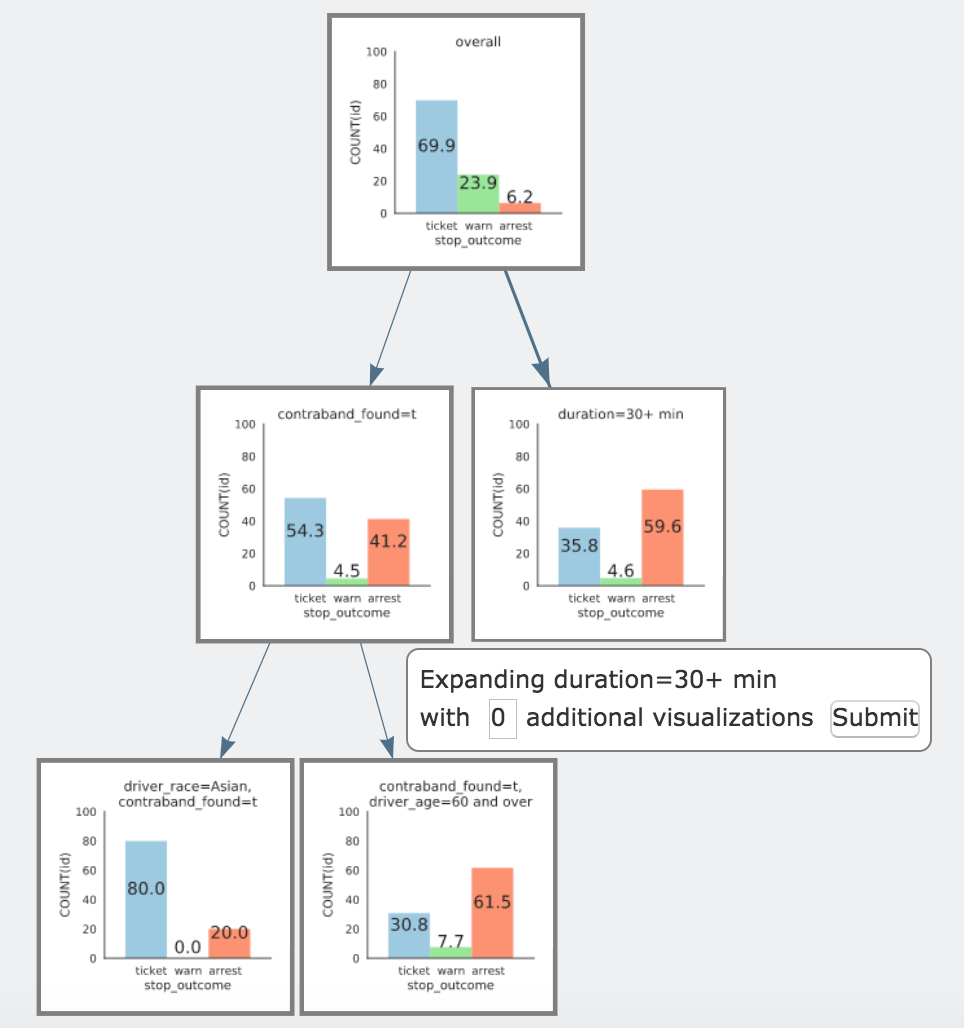
\includegraphics[width=0.43\linewidth]{figures/before_expansion2.png}
\raisebox{5\height}{
\includegraphics[width=0.05\linewidth]{figures/arrow_right.jpeg}}
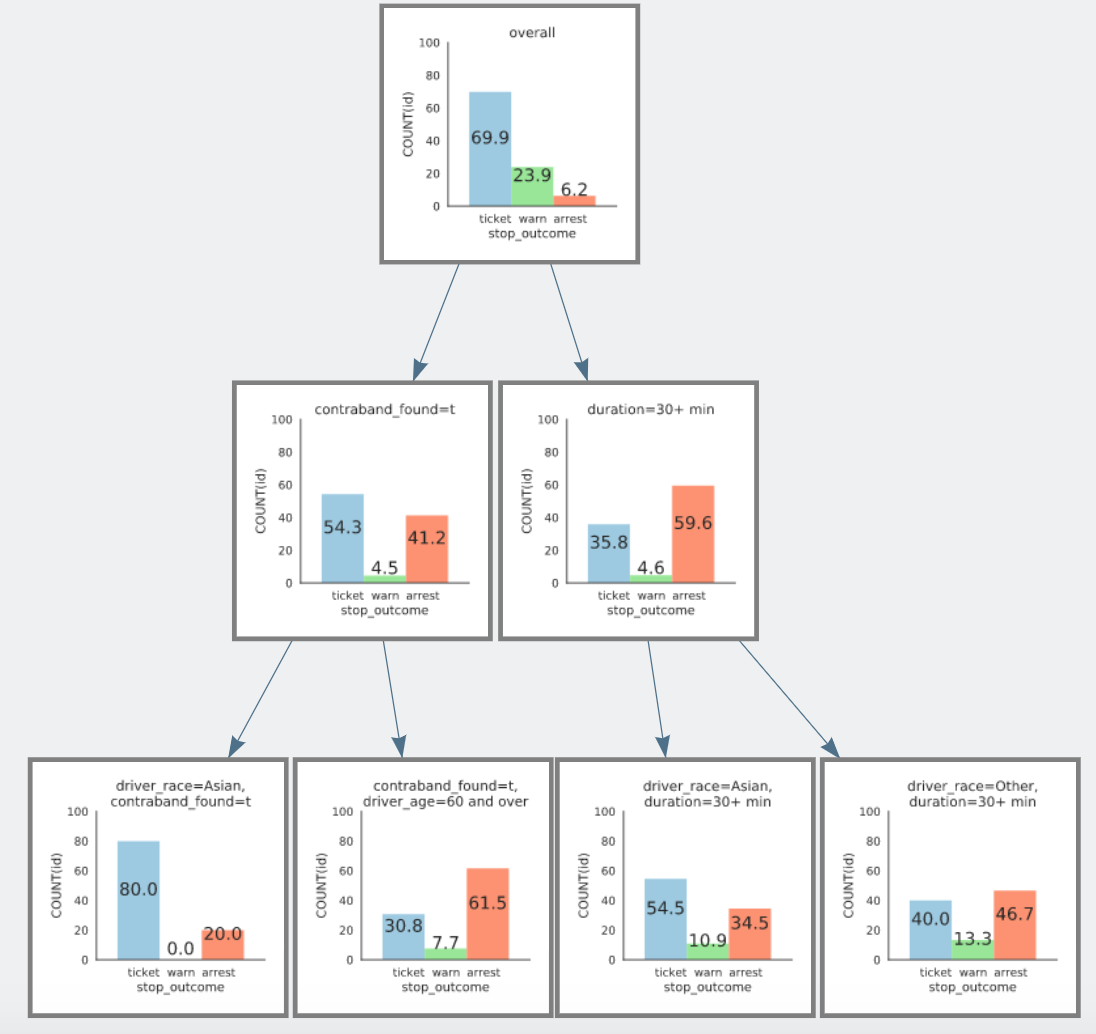
\includegraphics[width=0.49\linewidth]{figures/after_expansion3.png}
\caption{Left: Original k=5 dashboard with the duration=30+min visualization clicked. A pop-up is displayed to submit the request for additional summary visualizations to be generated. Right: Resulting dashboard after requesting for 2 more visualizations based on the visualization of interest.}
\label{fig:altroot_expansion}
\end{figure}
\subsection{Assistive tools for visualizing large lattices}
Due to the amount of space occupied by the hierarchical layout when the number of visualizations gets large, we have developed tools to help users navigate through difference parts of the dashboard interactively. 
\par \textbf{Navigation Minimap:}  When the user zooms in on the dashboard, an overview mini-map is shown on the upper right-hand side of the canvas to help users identify which region of the dashboard they are exploring, as shown in Figure \ref{fig:hover_minimap}. 
\par \textbf{Collapsed visualizations:} 
One observation that we found across several datasets was that many of the visualization attributes resulted in identical distributions. Apart from their attribute name, these visualizations are not very informative for the users, therefore, we offer an option to collapse these visualization, as demonstrated in Figure \ref{fig:collapse_demo}. A visualization can be collapsed if it has more than one redundant sibling and does not have any children. As shown in Figure \ref{fig:hover_minimap}, collapsed nodes can be easily identified by an orange border and the details of which visualizations are in the collapsed node are displayed when the user hovers over the visualization.
\begin{figure}[ht!]
\centering
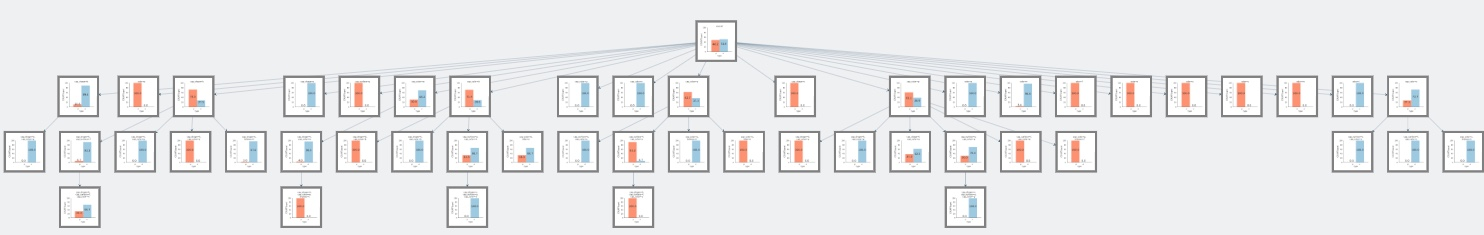
\includegraphics[width=\linewidth]{figures/k50_original.jpeg}
% \noindent\makebox[\linewidth]{\rule{\linewidth}{0.4pt}}
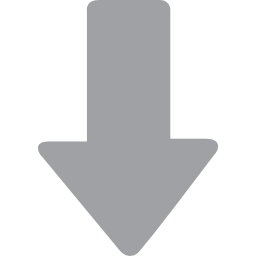
\includegraphics[width=0.05\linewidth]{figures/arrow_down.png}
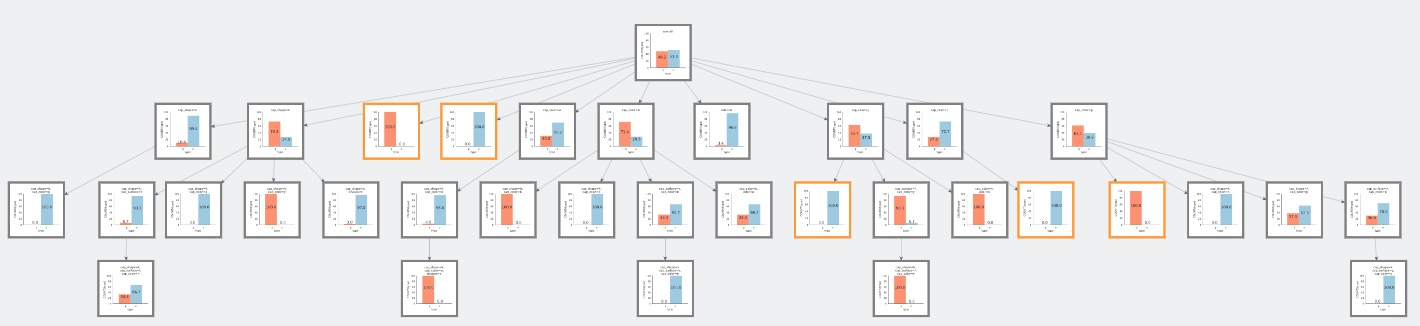
\includegraphics[width=\linewidth]{figures/k50_collapsed.jpeg}
\caption{An example of the k=50 dashboard for the mushroom dataset\footnote{\url{https://www.kaggle.com/uciml/mushroom-classification}}, which contains type =\{posionous, edible\} on the x-axis. The collapsed dashboard (bottom) removed 16 redundant visualizations from the original dashboard (top).}
\label{fig:collapse_demo}
\end{figure}

\begin{figure}[ht!]
\centering
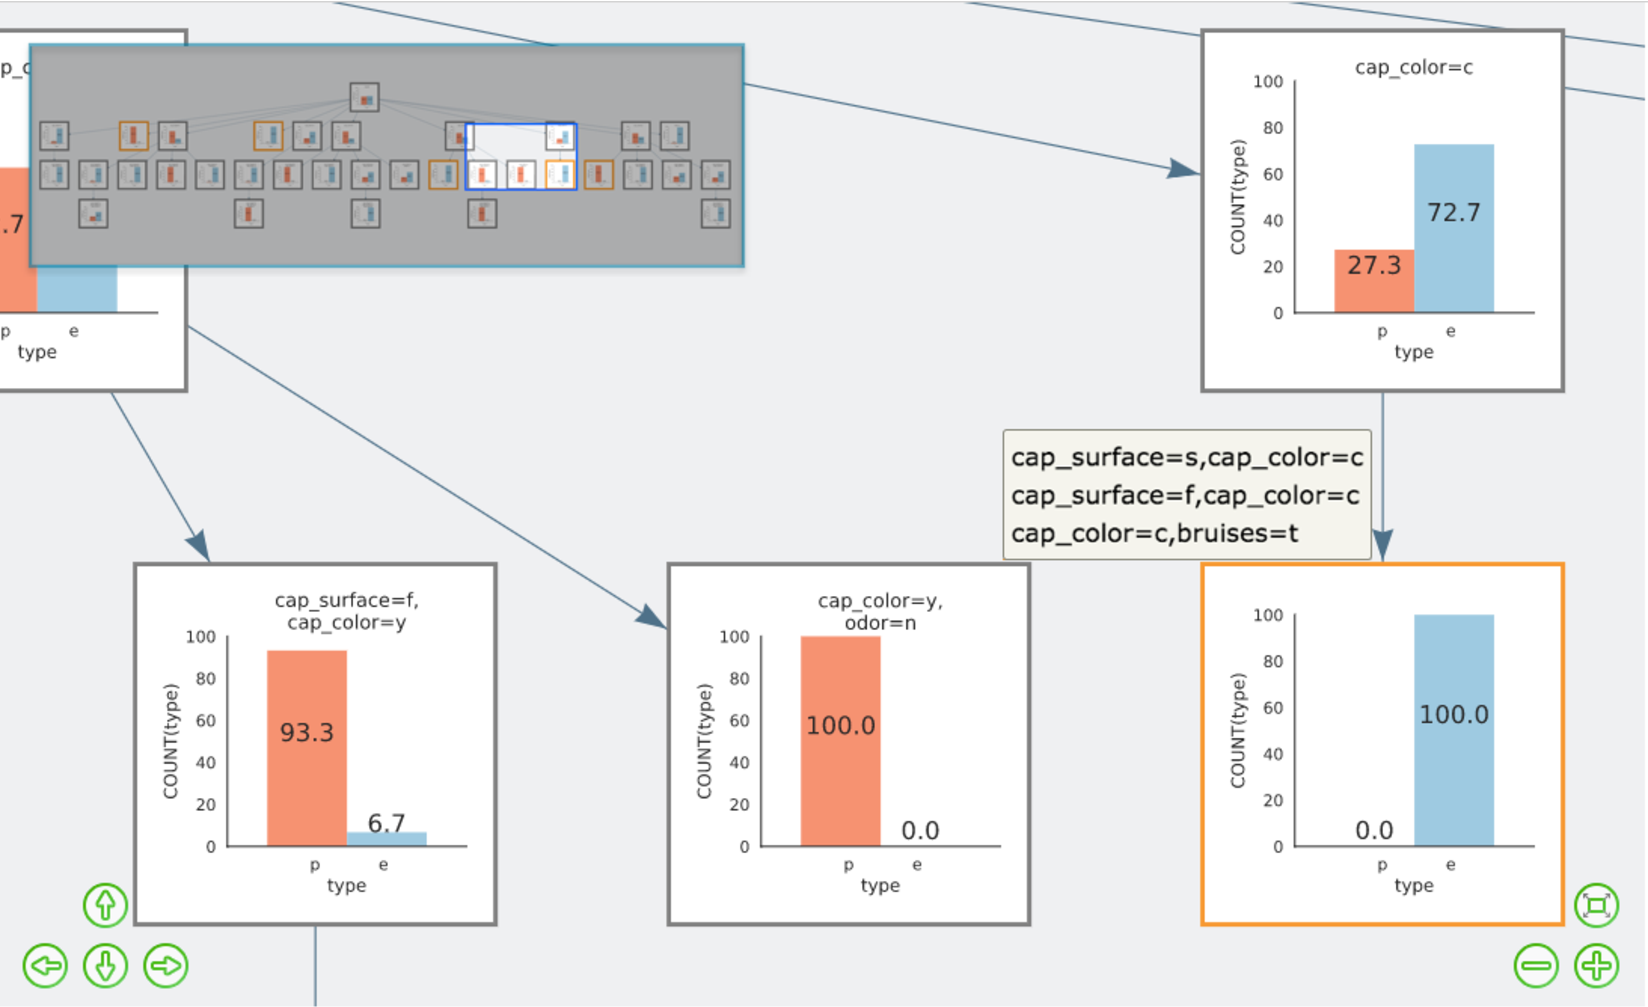
\includegraphics[width=\linewidth]{figures/minimap_cropped.pdf}
\caption{Zoomed-in version of Figure \ref{fig:collapse_demo} showing the labels of a collapsed visualization when user hovers over the visualization. The navigation minimap is shown in the top-left to help users navigate through the a large dashboard.}
\label{fig:hover_minimap}
\end{figure}
